\newpage\section{An{á}lisis sensor Aceler{ó}metro}

En este apartado abordaremos el análisis del sensor acelerómetro que es ampliamente utilizado para detectar cuando una persona sufre una caída; de acuerdo a la investigación se deberán responder las siguientes preguntas: ¿cómo determinamos qué una persona está cayendo?, ¿cuáles son los rangos en los que se establece que una persona sufrió una caída?, ¿cuáles son los motivos por los que se seleccionó el acelerómetro \textbf{MPU-6050}? y por último, ¿cuál es el funcionamiento y las características principales del acelerómetro \textbf{MPU-6050}?. \\

\subsection{Etapas de una caída}

Una caída comprende 4 etapas, en las cuales se observa una aceleración diferente y las etapas críticas tienden a ser los rangos de evaluación para definir si se sufrió o no dicha acción. A continuación, se describen dichas etapas \cite{cuarentaynueve}:

\begin{figure}[h]
	\centering
	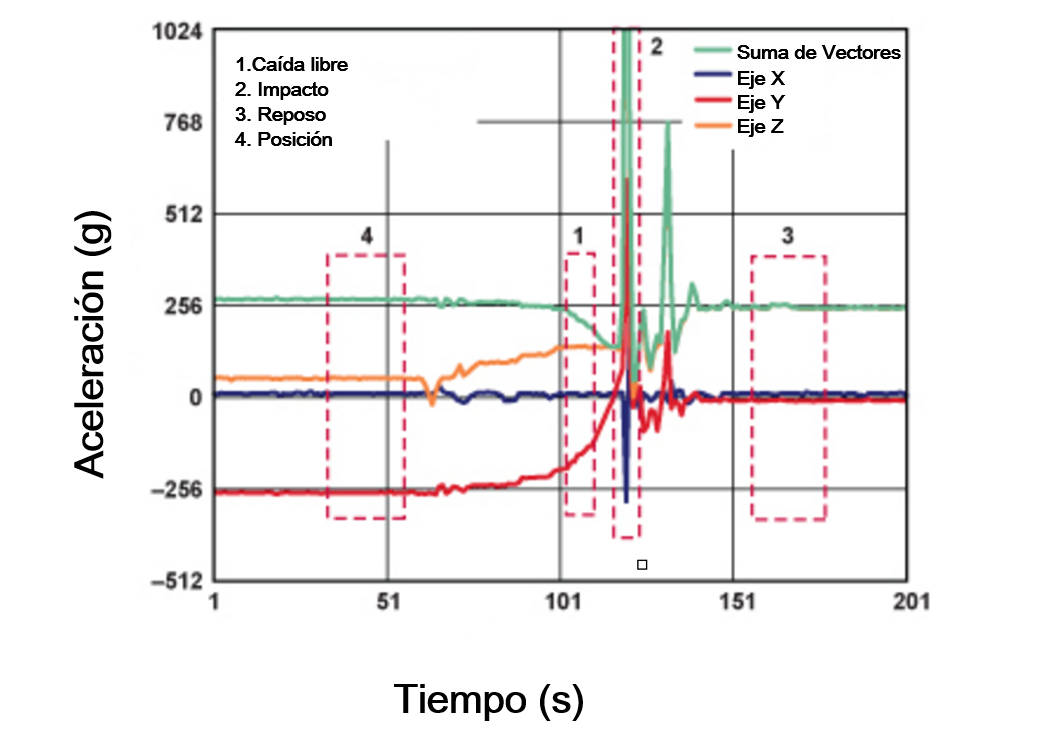
\includegraphics[scale=0.35]{analisis/imagenes/etapas_caida}
	\textbf{\caption{\small{Gráfica 2.1 Puntos de interés en la señal que muestra: (a) posturas al sufrir una caída y (b) actividades cotidianas \cite{cuarentaynueve}.}}}
	\label{fig:sensorcaida}
\end{figure}

\begin{itemize}
	\item \textbf{Caída libre}: Cuando una persona pierde el equilibrio se dirige hacia el suelo con un movimiento de caída libre y es justo donde se da el primer cambio en la señal; en esta etapa se contempla el fenómeno de gravedad y la suma vectorial de la aceleración se reflejará menor que 1g y mayor que $0g (1g > a > g)$. 
	\item \textbf{Impacto}: El cuerpo tendrá un choque con el suelo, pared u objeto, en esta etapa la señal tendrá un cambio significativo teniendo un pico muy elevado con valores en la aceleración de entre $2g \quad y \quad 12g$.
	\item \textbf{Reposo}: El cuerpo humano, después de caer y hacer impacto, no puede levantarse de inmediato; por lo que permanece en una posición inmóvil durante un período de tiempo (este puede ser corto o largo dependiendo de la gravedad de la caída).
	\item \textbf{Posición final}: Después de una caída, el cuerpo de la persona estará en una orientación diferente a la anterior, por lo que la aceleración estática en tres ejes será diferente de la situación inicial antes de la caída. Se hace un muestreo de la aceleración antes (muestreo inicial) y después (muestreo final) de la caída, se comparan los datos de muestreo y se evalúa; si la diferencia entre los datos de muestreo y supera un umbral de $0,7 g$ se declara como caída.
\end{itemize}

\subsection{Algoritmo basado en umbrales y orientación}

Simplemente se basa en detectar las cuatro etapas de las caídas: caída libre, impacto, reposo y posición final.	Se describirá el siguiente algoritmo el cual se abordará en este proyecto para detectar las caídas.

\begin{figure}[h]
	\centering
	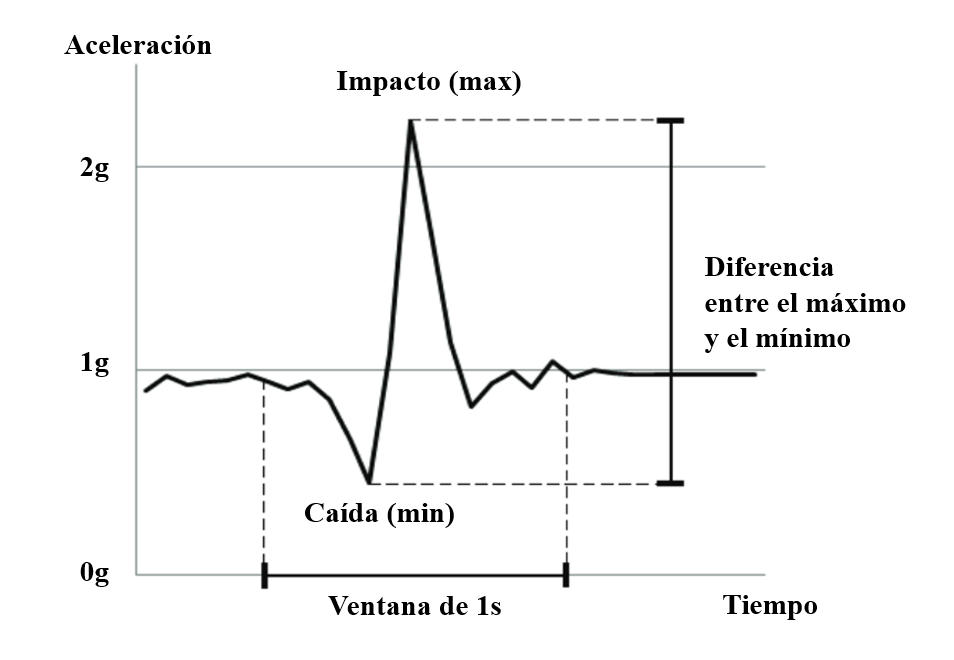
\includegraphics[scale=0.35]{analisis/imagenes/aceleracion}
	\textbf{\caption{\small{Gráfica 2.2 Patrón de la aceleración durante una caída \cite{cincuenta}.}}}
	\label{fig:sensorcaida2}
\end{figure}

\begin{enumerate}
	\item Un acelerómetro registra que una persona en reposo tiene de $1g$ (gravedad de la Tierra) de aceleración y durante la caída libre dicha aceleración tiende a 0 g. Cuando una persona comienza a caer, la aceleración disminuye de $1g \quad a \quad 0.5g$ aproximadamente (nunca se logra caída libre perfecta). 
	\item Tras el impacto con el suelo, se mide un alto y bajo aumento en la aceleración, lo cual nos da un pico muy largo.
	\item En el umbral, se utiliza la longitud del vector de aceleración, ignorando la dirección de la aceleración. En el lapso de un segundo se mide la aceleración máxima y mínima, si la diferencia entre estas aceleraciones: máxima y mínima es mayor de 1g y la máxima se produce después de la mínima, se declara que se ha producido una caída. 
	\item Sea $z$ el eje apuntando hacia abajo cuando la persona está de pie en posición vertical. El ángulo entre el vector de aceleración y el eje $z$, indica la orientación de la persona, y se calcula mediante la siguiente fórmula: 
\end{enumerate}

\begin{equation}
cos\varphi \equiv \frac{{\alpha}_{z}}{\sqrt{{{\alpha}_{x^2}+{\alpha}_{y^2}+{\alpha}_{z^2}}}}
\end{equation}

Puesto que cada persona tiene su postura característica y el acelerómetro puede no siempre ser usado exactamente de la misma manera, la orientación promedio de cada persona durante 15 segundos de caminar se mide como ${\varphi}_{0}$. Posteriormente, cuando se mide una nueva orientación $\varphi$, se normaliza como sigue: ${\varphi}_{norm} = \varphi – {\varphi}_{0}$. Una persona es considerada orientada hacia arriba, si $-30^{\circ} < {\varphi}_{norm} < 30^{\circ}$. Por lo cual, si se ha detectado una aceleración que supera el umbral como se ha descrito anteriormente, y la orientación de la persona durante 10 segundos no es en posición vertical, se declara que se ha producido una caída \cite{cincuenta}.

\subsection{Selección y tabla comparativa de acelerómetros}

El acelerómetro seleccionado fue el MPU-6050, de acuerdo a la investigación en la tabla comparativa, esto fue porque incluye un giroscopio, su tipo de interfaz es digital I$^{2}$C, el costo es promedio comparado con los demás, además de tener un diseño para el bajo consumo de energía, de estas características podemos resaltar que es ampliamente usado en: teléfonos inteligentes, tabletas y sensores portátiles. \\

\begin{table}
	\centering
	\begin{tabular}{|p{3cm}|p{2cm}|p{2cm}|p{2cm}|p{2cm}|}
		\hline
		\multicolumn{5}{|c|}{Tabla comparativa de acelerómetros} \\
		\cline{1-5} \hline
		\centering Modelo & \centering MPU-6050 &\centering ADXL345 & \centering MMA8451Q & \centering LIS331HH \\
		\tabularnewline
		\hline 
		Fabricante & Inven Sense & Analog Devices & Freescale & ST Microelectronics \\ \cline{1-5}
		\hline 
		Salida & Digital 8 bits & Digital de 12 bits & Digital 13 bits & Digital 16 bits \\ \cline{1-5}
		\hline
		Interfaz de comunicación & I2C & SPI, I2C & I2C & I2C \\ \cline{1-5}
		\hline
		Rango de medición & $\pm2g$, $\pm4g$, $\pm8g$, $\pm16g$ & $\pm16$ & $+/- 8g$ & $+/- 24g$ \\ \cline{1-5}
		\hline
		Dimensión & 4mm x 4mm x 0.9mm & 3mm x 5mm x 1mm & 3mm x 5mm x 1mm & 3mm x 5mm x 1mm \\ \cline{1-5}
		\hline
		Ejes & 3 & 3 & 3 & 3 \\ \cline{1-5}
		\hline
		Precisión & 1mg/LSB & 4 mg/LSB & 0.98 g/LSB & 3 mg/LSB (a +/-12g) \\ \cline{1-5}
		\hline
		Alimentación & 2.375V a 3.46V & 2V a 3.6V & 1.95V a 3.6V & 2.16V a 3.6V \\ \cline{1-5} 
		\hline
		Corriente Máxima & - & 40uA & 165uA & 10uA \\ \cline{1-5} 
		\hline
		Características adicionales & Incluye giroscopio & - & - & - \\ \cline{1-5} 
		\hline
		Frecuencia de muestreo & Hasta 400kHz & Hasta 3200 Hz & Hasta 800 Hz & Hasta 1 KHz \\ \cline{1-5} 
		\hline
		Rango de temperatura & -40$^\circ$C a +85$^\circ$C & -40$^\circ$C a +85$^\circ$C & -40$^\circ$C a +85$^\circ$C & -40$^\circ$C a +85$^\circ$C \\ \cline{1-5} 
		\hline
		Calibración & Programable & De Fábrica & De Fábrica & De Fábrica \\ \cline{1-5} 
		\hline
		Montaje superficial & si & si & si & si \\ \cline{1-5} 
		\hline
		Costo & \$3.99 & \$6.93 & \$2.16 & \$5.97 \\ \cline{1-5} 
		\hline
	\end{tabular}
	\centering\textbf{\caption{\small{\textbf{Escenarios y posturas en los que el acelerómetro realizará muestreo.}}}}
\end{table}

\subsection{Características, especificaciones y funcionamiento interno del acelerómetro MPU-6050}

El acelerómetro MPU-6050 cuenta con un acelerómetro y un giroscopio internos, este dispositivo es altamente usado en aplicaciones basadas en video, estabilización de imágenes, seguridad en autenticación, reconocimiento de gestos, control de movimiento, sensores para la salud, sensores para condición física, sensores para deporte y juguetes. En el siguiente apartado se mostrarán las características, diagrama a bloques y la descripción con las que cuenta dicho dispositivo.

\begin{itemize}
	\item \textbf{Características}
\end{itemize}

En la tabla 2.34 se marcarán las características principales para el dispositivo. \\

\begin{table}
	\begin{tabular}{|p{4cm}|p{4cm}|p{4cm}|}
		\hline 
		\centering Acelerómetro & \centering Giroscopio & \centering Adicionales \\ 
		\tabularnewline
		\hline 
		Salida digital de 3 ejes: X, Y y Z, con un rango de escala programable por el usuario de: $\pm2g$, $\pm4g$, $\pm8g$ y $\pm16g$. & Salida digital de 3 ejes: X, Y y Z, con un rango de escala programable por el usuario de $\pm250$, $\pm500$, $\pm1.000$ y $\pm2.000g/seg.$ & Procesador digital de movimiento (DMP) \\ 
		\hline 
		Convertidores analógico digital (ADC) de 16 bits permiten el muestreo simultáneo. & Convertidores analógico digital (ADC) de 16 bits que permiten el muestreo simultáneo. & Auxiliar bus I2C maestro para leer los datos de los sensores externos. \\ 
		\hline 
		Baja potencia de: 10$\mu$A en 1.25Hz, 20$\mu$A a 5Hz, 20Hz a 60mA, 110$\mu$A a 40Hz. & La baja frecuencia mejora el rendimiento y disminuye de ruido. & Rango de tensión de alimentación VDD 2.375V-3.46V. \\  
		\hline 
		Detección de orientación y señalización. & Estabilidad de la polarización y sensibilidad a la temperatura mejorada reduce la necesidad de calibración del usuario. & Tensión de referencia VLOGIC flexible soporta múltiples voltajes de interfaz I2C. \\ 
		\hline 
		Detección de Toque. & Filtro de paso bajo y paso alto digitalmente programables. & Un búfer de 1024 bytes FIFO reduce el consumo de energía al permitir que el procesador principal para lea los datos en ráfagas y luego entra en un modo de baja potencia para que la MPU recoja más datos. \\ 
		\hline 
		Corriente de operación 500$\mu$A. & Corriente de operación 3.6mA. & Salida digital del sensor de temperatura. \\ 
		\hline 
		- & Corriente de espera 5$\mu$A. & - \\
		\hline
		Interrupciones programables por el usuario. & Factor de escala de sensibilidad calibrado de fábrica. & - \\
		\hline
		Autocomprobación del usuario. & Autocomprobación del usuario. & - \\
		\hline
	\end{tabular} 
\textbf{\caption{\small{\textbf{Características principales del sensor acelerómetro MPU-6050.}}}}
\end{table}

\newpage
\begin{itemize}
	\item \textbf{Diagrama a bloques}
\end{itemize}

\begin{figure}[h]
	\centering
	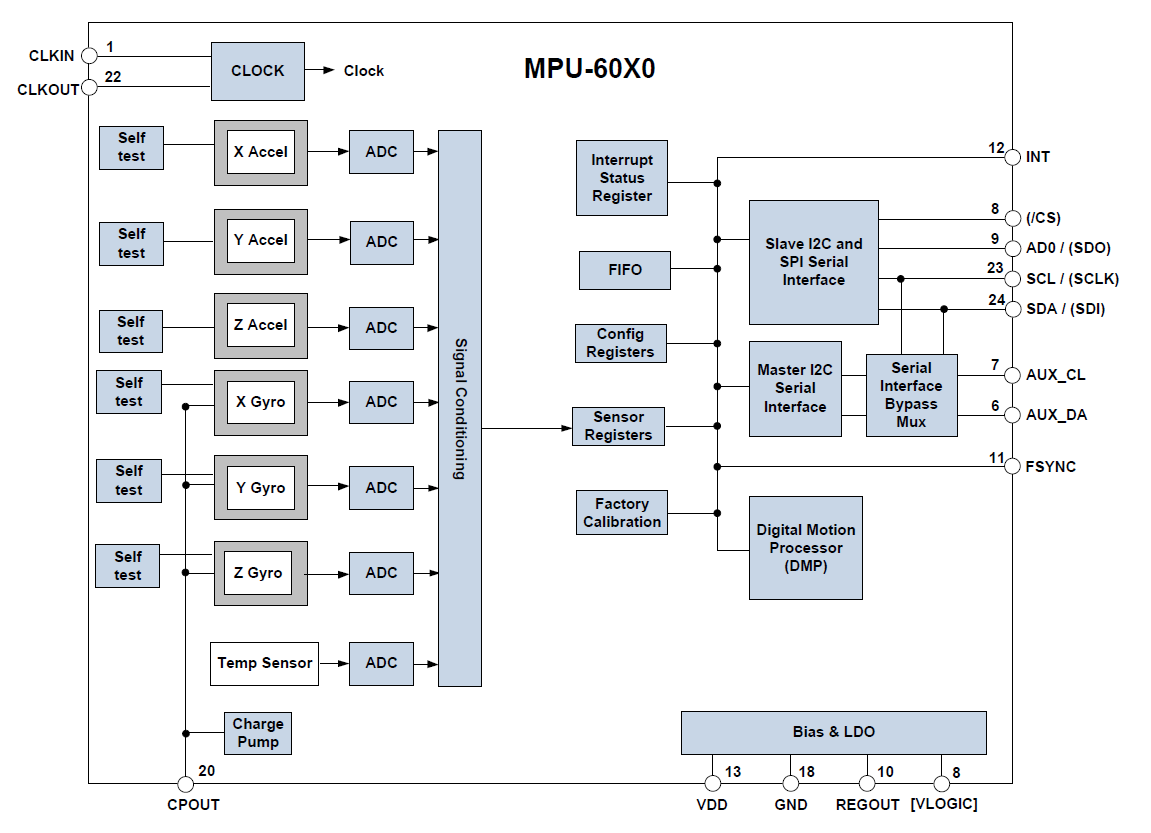
\includegraphics[scale=0.35]{analisis/imagenes/diagrama_acelerometro}
	\textbf{\caption{\small{Diagrama a bloques del acelerómetro MPU-6050.}}}
	\label{fig:DiagramaAcelerometro}
\end{figure}

En el siguiente diagrama a bloques que se muestra en la figura 2.10, podemos observar los módulos de los que está compuesto el acelerómetro MPU-6050. Este dispositivo comprende 6 ejes, 3 del acelerómetro y 3 del giroscopio; 6 convertidores analógicos a digital (ADC) de 16 bits, de igual manera 3 para el acelerómetro y 3 para el giroscopio; un procesador digital de movimiento (DMP), un bus de interfaz dedicado $I^2C$ a 400kHz y un sensor de temperatura. Además de los bloques anteriores podemos resaltar que maneja circuitería CMOS, sus medidas son: 4x4x0.9mm, lo cual permite más rendimiento y menos ruido además de un costo mucho más bajo. 
